\documentclass{article}%
\usepackage[T1]{fontenc}%
\usepackage[utf8]{inputenc}%
\usepackage{lmodern}%
\usepackage{textcomp}%
\usepackage{lastpage}%
\usepackage{graphicx}%
\usepackage{float}%
\usepackage{graphicx}%
%
\title{Research Keywords Analysis}%
\author{Pascal Friederich}%
\date{\today}%
%
\begin{document}%
\normalsize%
\maketitle%
\section{Introduction}%
\label{sec:Introduction}%
This document presents a comprehensive analysis of research concepts.

%
\section{Keyword Analysis}%
\label{sec:KeywordAnalysis}%


\begin{figure}[H]%
\centering%
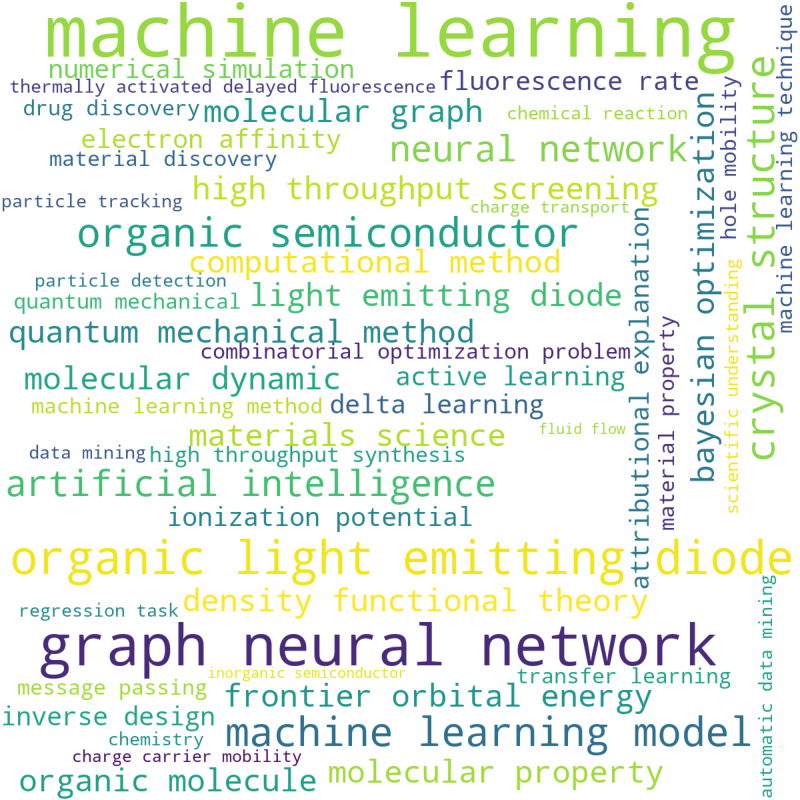
\includegraphics[width=0.8\textwidth]{wordcloud.png}%
\caption{Wordcloud of interesting concepts (count > 2).}%
\end{figure}

%


\begin{figure}[H]%
\centering%
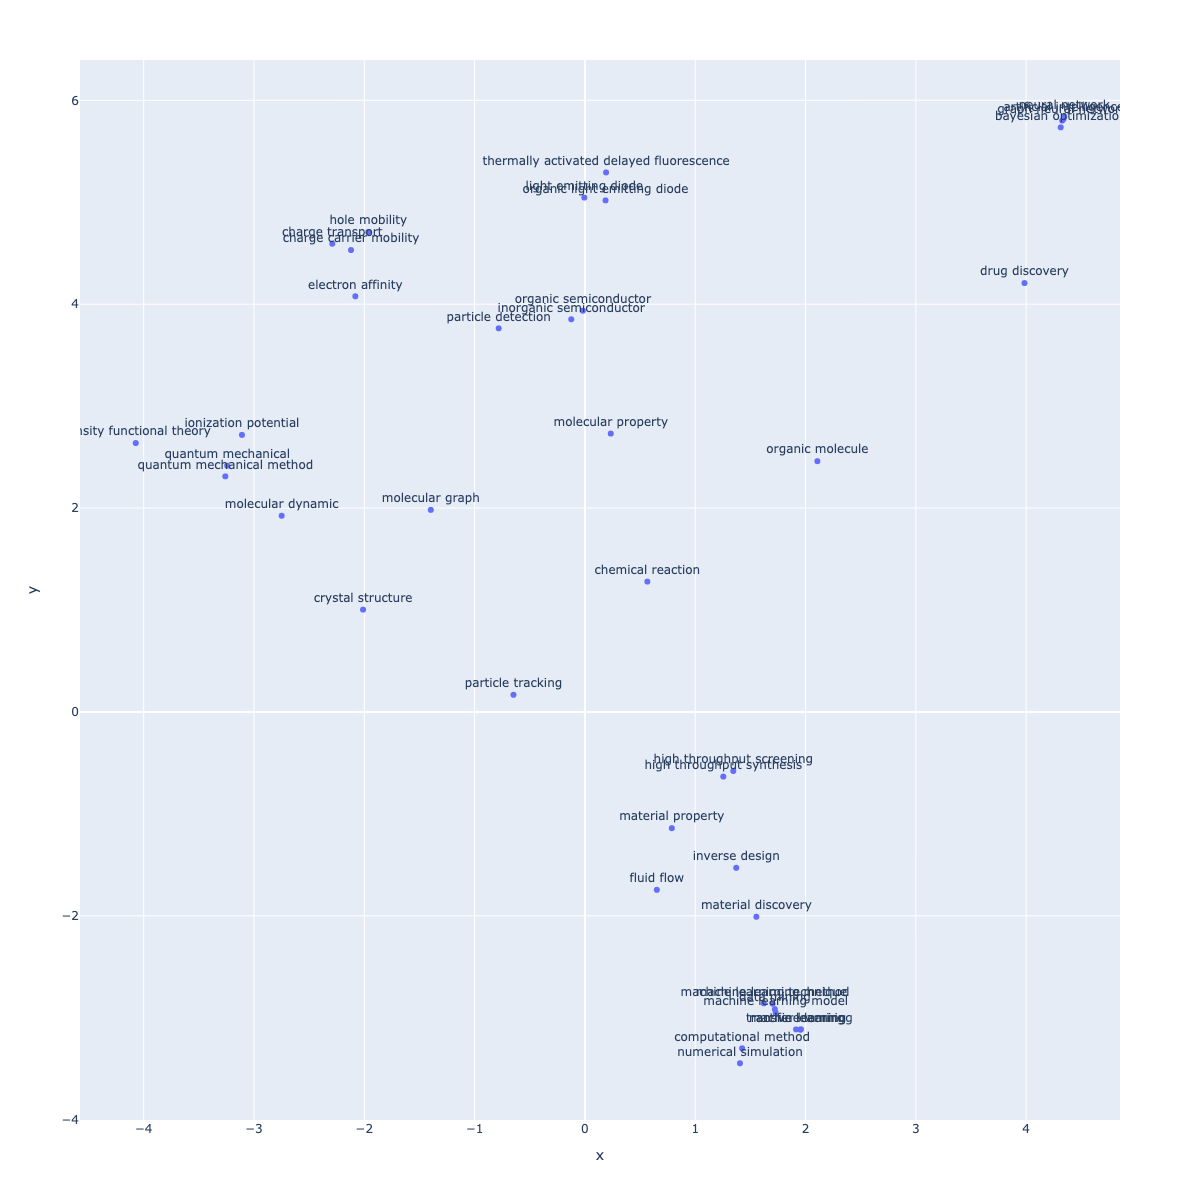
\includegraphics[width=0.8\textwidth]{embeddings_map.pdf}%
\caption{2D Embeddings Map of interesting concepts.}%
\end{figure}

%
The following concepts were extracted using a fine{-}tuned version of 'LlaMa{-}2{-}13B' from abstracts of your published papers (count > 2):\newline%
%
\begin{itemize}%
\item%
machine learning: (14)%
\item%
graph neural network: (8)%
\item%
organic light emitting diode: (7)%
\item%
organic semiconductor: (5)%
\item%
machine learning model: (5)%
\item%
crystal structure: (5)%
\item%
artificial intelligence: (4)%
\item%
neural network: (4)%
\item%
bayesian optimization: (3)%
\item%
light emitting diode: (3)%
\item%
density functional theory: (3)%
\item%
frontier orbital energy: (3)%
\item%
molecular graph: (3)%
\item%
molecular dynamic: (3)%
\item%
quantum mechanical method: (3)%
\item%
high throughput screening: (3)%
\item%
molecular property: (3)%
\item%
materials science: (3)%
\item%
computational method: (3)%
\item%
organic molecule: (3)%
\item%
numerical simulation: (2)%
\item%
active learning: (2)%
\item%
attributional explanation: (2)%
\item%
delta learning: (2)%
\item%
electron affinity: (2)%
\item%
ionization potential: (2)%
\item%
fluorescence rate: (2)%
\item%
inverse design: (2)%
\item%
combinatorial optimization problem: (2)%
\item%
hole mobility: (2)%
\item%
drug discovery: (2)%
\item%
high throughput synthesis: (2)%
\item%
material discovery: (2)%
\item%
machine learning technique: (2)%
\item%
machine learning method: (2)%
\item%
quantum mechanical: (2)%
\item%
transfer learning: (2)%
\item%
message passing: (2)%
\item%
material property: (2)%
\item%
thermally activated delayed fluorescence: (2)%
\item%
chemistry: (2)%
\item%
chemical reaction: (2)%
\item%
regression task: (2)%
\item%
scientific understanding: (2)%
\item%
particle detection: (2)%
\item%
particle tracking: (2)%
\item%
automatic data mining: (2)%
\item%
data mining: (2)%
\item%
charge carrier mobility: (2)%
\item%
charge transport: (2)%
\item%
inorganic semiconductor: (2)%
\item%
fluid flow: (2)%
\end{itemize}

%
\section{Suggestions of Research Directions}%
\label{sec:SuggestionsofResearchDirections}%
\subsection{Own Concepts Combinations (Best 25)}%
\label{subsec:OwnConceptsCombinations(Best25)}%
\begin{itemize}%
\item%
\textbf{sustainable energy conversion} and high entropy alloy: 1.0%
\item%
\textbf{basic principle} and crystal structure: 1.0%
\item%
\textbf{electronic structure} and numerical simulation: 1.0%
\item%
\textbf{data driven method} and solar cell: 1.0%
\item%
\textbf{high throughput approach} and physicochemical property: 1.0%
\item%
\textbf{virtual model} and molecular dynamic simulation: 1.0%
\item%
\textbf{quantum mechanical computation} and high entropy alloy: 1.0%
\item%
\textbf{atomistic simulation} and electronic structure: 1.0%
\item%
\textbf{synthesis parameter} and surface area: 1.0%
\item%
\textbf{machine learning method} and surface area: 1.0%
\item%
\textbf{quantitative structure property relationship} and material property: 1.0%
\item%
\textbf{graph model} and physicochemical property: 1.0%
\item%
\textbf{property requirement} and surface area: 0.9999%
\item%
\textbf{superconducting material} and atomistic simulation: 0.9999%
\item%
\textbf{symmetry operation} and optoelectronic application: 0.9999%
\item%
\textbf{accelerated stress test} and artificial neural network: 0.9999%
\item%
\textbf{high throughput} and crystal structure: 0.9999%
\item%
\textbf{data mining} and optoelectronic application: 0.9999%
\item%
\textbf{soft material} and artificial neural network: 0.9999%
\item%
\textbf{charge carrier} and atomistic simulation: 0.9998%
\item%
\textbf{deep neural network} and density functional theory: 0.9998%
\item%
\textbf{computational chemistry} and molecular dynamic simulation: 0.9998%
\item%
\textbf{numerical simulation} and metal organic framework: 0.9998%
\item%
\textbf{synthesis condition} and physicochemical property: 0.9997%
\item%
\textbf{quantum chemistry} and charge transport: 0.9997%
\end{itemize}

%
\subsection{Other Concepts Combinations (Best 25)}%
\label{subsec:OtherConceptsCombinations(Best25)}%
\begin{itemize}%
\item%
\textbf{organic photovoltaic} and additive manufacturing: 1.0%
\item%
\textbf{density functional theory method} and scanning electron microscope: 1.0%
\item%
\textbf{cost advantage} and transmission electron microscopy: 1.0%
\item%
\textbf{structural search} and scanning electron microscopy: 1.0%
\item%
\textbf{coating design} and graphene oxide: 1.0%
\item%
\textbf{quasiparticle energy} and ultimate tensile strength: 1.0%
\item%
\textbf{machine learning} and mathematical model: 1.0%
\item%
\textbf{particle tracking} and surface modification: 1.0%
\item%
\textbf{drag coefficient} and energy dispersive spectroscopy: 1.0%
\item%
\textbf{site energy} and residual stress: 1.0%
\item%
\textbf{clean energy} and tensile strength: 1.0%
\item%
\textbf{ionization energy} and tensile strength: 1.0%
\item%
\textbf{optimization problem} and titanium alloy: 1.0%
\item%
\textbf{organic light emitting diode} and hydrothermal method: 1.0%
\item%
\textbf{transition energy} and CS: 1.0%
\item%
\textbf{quantum chemistry} and solid solution strengthening: 1.0%
\item%
\textbf{optimization problem} and crystallite size: 1.0%
\item%
\textbf{organic photovoltaic} and laser powder bed fusion: 1.0%
\item%
\textbf{organic material} and lattice structure: 1.0%
\item%
\textbf{critical temperature} and titanium alloy: 1.0%
\item%
\textbf{data augmentation} and mechanical strength: 1.0%
\item%
\textbf{triplet state} and precipitation strengthening: 1.0%
\item%
\textbf{thermally activated delayed fluorescence} and x ray diffraction: 1.0%
\item%
\textbf{organic emitter} and scanning electron microscopy: 1.0%
\item%
\textbf{solution processing} and digital image correlation: 1.0%
\end{itemize}

%
\section{Top 20 Concepts with most highest scored connections to your own concepts (score >= 0.999)}%
\label{sec:Top20Conceptswithmosthighestscoredconnectionstoyourownconcepts(score>=0.999)}%
\subsection{Recommendation: photoluminescence spectroscopy}%
\label{subsec:Recommendationphotoluminescencespectroscopy}%
To be combined with your work on:%
\begin{itemize}%
\item%
electroluminescent property: 0.9999%
\item%
molecular aggregation: 0.9997%
\item%
ionization potential: 0.9997%
\item%
structural search: 0.9996%
\item%
high throughput screening: 0.9994%
\item%
quantum mechanical: 0.9991%
\item%
metal organic framework: 0.9991%
\item%
quantum mechanical method: 0.999%
\item%
particle image: 0.999%
\end{itemize}

%
\subsection{Recommendation: tensile strength}%
\label{subsec:Recommendationtensilestrength}%
To be combined with your work on:%
\begin{itemize}%
\item%
clean energy: 1.0%
\item%
ionization energy: 1.0%
\item%
hybrid system: 0.9999%
\item%
physical science: 0.9998%
\item%
finite element computation: 0.9996%
\item%
particle tracking: 0.9996%
\item%
microscopic simulation: 0.9995%
\item%
dielectric permittivity: 0.999%
\end{itemize}

%
\subsection{Recommendation: laser power}%
\label{subsec:Recommendationlaserpower}%
To be combined with your work on:%
\begin{itemize}%
\item%
inverse design: 1.0%
\item%
density functional theory: 1.0%
\item%
force field: 0.9999%
\item%
bulk phase: 0.9997%
\item%
classical molecular dynamic simulation: 0.9995%
\item%
molecular catalyst: 0.9994%
\item%
particle tracking: 0.9993%
\item%
site energy: 0.9993%
\end{itemize}

%
\subsection{Recommendation: scanning electron microscopy}%
\label{subsec:Recommendationscanningelectronmicroscopy}%
To be combined with your work on:%
\begin{itemize}%
\item%
structural search: 1.0%
\item%
organic emitter: 1.0%
\item%
force field: 0.9999%
\item%
material property prediction: 0.9995%
\item%
site energy: 0.9992%
\item%
kinetic monte carlo: 0.9991%
\item%
optimization problem: 0.9991%
\end{itemize}

%
\subsection{Recommendation: electron backscattered diffraction}%
\label{subsec:Recommendationelectronbackscattereddiffraction}%
To be combined with your work on:%
\begin{itemize}%
\item%
simulated data: 1.0%
\item%
optical readout: 1.0%
\item%
coating design: 1.0%
\item%
surface area: 0.9999%
\item%
drug discovery: 0.9999%
\item%
triplet state: 0.9997%
\item%
bayesian optimization: 0.9994%
\end{itemize}

%
\subsection{Recommendation: physicochemical property}%
\label{subsec:Recommendationphysicochemicalproperty}%
To be combined with your work on:%
\begin{itemize}%
\item%
high throughput approach: 1.0%
\item%
graph model: 1.0%
\item%
synthesis condition: 0.9997%
\item%
particle detection: 0.9996%
\item%
theoretical chemistry: 0.9995%
\item%
critical temperature: 0.9993%
\end{itemize}

%
\subsection{Recommendation: digital image correlation}%
\label{subsec:Recommendationdigitalimagecorrelation}%
To be combined with your work on:%
\begin{itemize}%
\item%
solution processing: 1.0%
\item%
data mining: 0.9999%
\item%
computational power: 0.9998%
\item%
high throughput synthesis: 0.9996%
\item%
calibrated model: 0.9994%
\item%
ionization potential: 0.9993%
\end{itemize}

%
\subsection{Recommendation: strength enhancement}%
\label{subsec:Recommendationstrengthenhancement}%
To be combined with your work on:%
\begin{itemize}%
\item%
high entropy oxide: 1.0%
\item%
time scale: 0.9999%
\item%
material composition: 0.9999%
\item%
cost advantage: 0.9996%
\item%
quantum mechanical treatment: 0.9993%
\item%
fluorescent emitter: 0.9992%
\end{itemize}

%
\subsection{Recommendation: annealing temperature}%
\label{subsec:Recommendationannealingtemperature}%
To be combined with your work on:%
\begin{itemize}%
\item%
organic molecule: 1.0%
\item%
material property prediction: 0.9999%
\item%
uv vis spectroscopy: 0.9993%
\item%
coating design: 0.9993%
\item%
transition energy: 0.9993%
\item%
charge carrier: 0.9991%
\end{itemize}

%
\subsection{Recommendation: antibacterial activity}%
\label{subsec:Recommendationantibacterialactivity}%
To be combined with your work on:%
\begin{itemize}%
\item%
high entropy alloy: 0.9999%
\item%
material composition: 0.9999%
\item%
numerical simulation: 0.9998%
\item%
drag coefficient: 0.9997%
\item%
small molecule: 0.9993%
\item%
element combination: 0.9992%
\end{itemize}

%
\subsection{Recommendation: bond strength}%
\label{subsec:Recommendationbondstrength}%
To be combined with your work on:%
\begin{itemize}%
\item%
machine learning technique: 0.9999%
\item%
organic molecule: 0.9997%
\item%
physicochemical property: 0.9996%
\item%
inorganic semiconductor: 0.9994%
\item%
phenolic compound: 0.9994%
\item%
cost advantage: 0.9993%
\end{itemize}

%
\subsection{Recommendation: solar cell}%
\label{subsec:Recommendationsolarcell}%
To be combined with your work on:%
\begin{itemize}%
\item%
data driven method: 1.0%
\item%
triangular lattice: 0.9997%
\item%
optimization problem: 0.9997%
\item%
image quality: 0.9996%
\item%
computational power: 0.9993%
\end{itemize}

%
\subsection{Recommendation: optoelectronic application}%
\label{subsec:Recommendationoptoelectronicapplication}%
To be combined with your work on:%
\begin{itemize}%
\item%
symmetry operation: 0.9999%
\item%
data mining: 0.9999%
\item%
cost advantage: 0.9996%
\item%
machine learning technique: 0.9991%
\item%
computer science: 0.9991%
\end{itemize}

%
\subsection{Recommendation: solid solution strengthening}%
\label{subsec:Recommendationsolidsolutionstrengthening}%
To be combined with your work on:%
\begin{itemize}%
\item%
quantum chemistry: 1.0%
\item%
multiscale modeling: 1.0%
\item%
simulated data: 1.0%
\item%
computer science: 0.9999%
\item%
calibrated model: 0.9998%
\end{itemize}

%
\subsection{Recommendation: crystallite size}%
\label{subsec:Recommendationcrystallitesize}%
To be combined with your work on:%
\begin{itemize}%
\item%
optimization problem: 1.0%
\item%
graph model: 0.9999%
\item%
post processing: 0.9999%
\item%
electroluminescent property: 0.9996%
\item%
simulated data: 0.9993%
\end{itemize}

%
\subsection{Recommendation: laser powder bed fusion}%
\label{subsec:Recommendationlaserpowderbedfusion}%
To be combined with your work on:%
\begin{itemize}%
\item%
organic photovoltaic: 1.0%
\item%
graph model: 1.0%
\item%
artificial neural network: 1.0%
\item%
critical temperature: 0.9999%
\item%
site energy: 0.9991%
\end{itemize}

%
\subsection{Recommendation: energy density}%
\label{subsec:Recommendationenergydensity}%
To be combined with your work on:%
\begin{itemize}%
\item%
cost advantage: 1.0%
\item%
surface science: 0.9999%
\item%
computer science: 0.9994%
\item%
graph model: 0.9993%
\item%
convolutional neural network: 0.9991%
\end{itemize}

%
\subsection{Recommendation: MoS2}%
\label{subsec:RecommendationMoS2}%
To be combined with your work on:%
\begin{itemize}%
\item%
triangular lattice: 1.0%
\item%
bulk phase: 1.0%
\item%
graph neural network: 1.0%
\item%
solution processing: 0.9999%
\item%
molecular catalyst: 0.9995%
\end{itemize}

%
\subsection{Recommendation: corrosion resistance}%
\label{subsec:Recommendationcorrosionresistance}%
To be combined with your work on:%
\begin{itemize}%
\item%
computational method: 1.0%
\item%
quasiparticle energy: 1.0%
\item%
particle tracking velocimetry: 0.9999%
\item%
quantum mechanical: 0.9993%
\item%
density functional theory method: 0.9992%
\end{itemize}

%
\subsection{Recommendation: low angle grain boundary}%
\label{subsec:Recommendationlowanglegrainboundary}%
To be combined with your work on:%
\begin{itemize}%
\item%
metal dissolution: 1.0%
\item%
bulk phase: 0.9999%
\item%
computational power: 0.9999%
\item%
high throughput approach: 0.9996%
\item%
machine learning model: 0.999%
\end{itemize}

%
\section{Map of Materials Science}%
\label{sec:MapofMaterialsScience}%


\begin{figure}[H]%
\centering%
\includegraphics[width=0.8\textwidth]{map_of_materials_science.pdf}%
\caption{Map of Materials Science with important landmarks}%
\end{figure}

%
\section{Used Papers}%
\label{sec:UsedPapers}%
The following papers were considered for concept extraction:%
\begin{itemize}%
\item%
Bayesian optimization approach to quantify the effect of input parameter uncertainty on predictions of numerical physics simulations%
\item%
Active learning for excited states dynamics simulations to discover molecular degradation pathways%
\item%
Navigating the Unkown With AI: Multiobjective Bayesian Optimization of Non{-}Noble Acidic OER Catalysts%
\item%
Quantifying the Intrinsic Usefulness of Attributional Explanations for Graph Neural Networks with Artificial Simulatability Studies%
\item%
MEGAN: Multi{-}Explanation Graph Attention Network%
\item%
Contextualized Policy Recovery: Modeling and Interpreting Medical Decisions with Adaptive Imitation Learning%
\item%
Interpretable delta{-}learning of GW quasiparticle energies from GGA{-}DFT%
\item%
Artificial Design of Organic Emitters via a Genetic Algorithm Enhanced by a Deep Neural Network%
\item%
The Role of Experimental Noise in a Hybrid Classical{-}Molecular Computer to Solve Combinatorial Optimization Problems%
\item%
Modeling Charge Transport in Organic Semiconductors Using Neural Network Based Hamiltonians and Forces%
\item%
Mitigating Molecular Aggregation in Drug Discovery with Predictive Insights from Explainable AI%
\item%
An integrated system built for small{-}molecule semiconductors via high{-}throughput approaches%
\item%
What is missing in autonomous discovery: Open challenges for the community%
\item%
Lattice Metamaterials with Mesoscale Motifs: Exploration of Property Charts by Bayesian Optimization%
\item%
Neural networks trained on synthetically generated crystals can extract structural information from ICSD powder X{-}ray diffractograms%
\item%
Accurate GW frontier orbital energies of 134 kilo molecules%
\item%
Connectivity Optimized Nested Graph Networks for Crystal Structures%
\item%
High‐Throughput Synthesis and Machine Learning Assisted Design of Photodegradable Hydrogels%
\item%
Predicting reaction barriers of hydrogen atom transfer in proteins%
\item%
Functional Material Systems Enabled by Automated Data Extraction and Machine Learning%
\item%
Carbazole{-}substituted benzobisoxazoles: near{-}UV fluorescent emitters and ambipolar hosts for organic light{-}emitting diodes%
\item%
Synthesis and Characterization of High‐Entropy CrMoNbTaVW Thin Films Using High‐Throughput Methods%
\item%
3DSC {-} A New Dataset of Superconductors Including Crystal Structures%
\item%
Graph neural networks for materials science and chemistry%
\item%
Actively Learning Costly Reward Functions for Reinforcement Learning%
\item%
Graph neural networks to learn joint representations of disjoint molecular graphs%
\item%
SELFIES and the future of molecular string representations%
\item%
On scientific understanding with artificial intelligence%
\item%
Particle detection by means of neural networks and synthetic training data refinement in defocusing particle tracking velocimetry%
\item%
28‐1: Invited Paper: Bottom‐Up OLED Development by Virtual Design: Systematic Elimination of Performance Bottlenecks Using a Microscopic Simulation Approach%
\item%
Vorhersage der MOF‐Synthese durch automatisches Data‐Mining und maschinelles Lernen%
\item%
MOF Synthesis Prediction Enabled by Automatic Data Mining and Machine Learning%
\item%
Charge Transfer Simulations using Hamiltonian Elements and Forces from Neural Networks%
\item%
Updated Calibrated Model for the Prediction of Molecular Frontier Orbital Energies and Its Application to Boron Subphthalocyanines%
\item%
A comprehensive discovery platform for organophosphorus ligands for catalysis%
\item%
De novo calculation of the charge carrier mobility in amorphous small molecule organic semiconductors%
\item%
Fast Generation of Machine Learning{-}Based Force Fields for Adsorption Energies%
\item%
Phase–Property Diagrams for Multicomponent Oxide Systems toward Materials Libraries%
\item%
Particle Detection by means of Machine Learning in Defocusing PTV%
\item%
Graph neural networks in TensorFlow{-}Keras with RaggedTensor representation (kgcnn)%
\item%
Neural message passing on high order paths%
\item%
Machine{-}learned potentials for next{-}generation matter simulations%
\item%
Computing Charging and Polarization Energies of Small Organic Molecules Embedded into Amorphous Materials with Quantum Accuracy%
\item%
Organic molecules with inverted gaps between first excited singlet and triplet states and appreciable fluorescence rates%
\item%
Analyzing dynamical disorder for charge transport in organic semiconductors via machine learning%
\item%
Scientific intuition inspired by machine learning{-}generated hypotheses%
\item%
A molecular computing approach to solving optimization problems via programmable microdroplet arrays%
\item%
Photochemical Aging of Levitated Aqueous Brown Carbon Droplets%
\item%
High{-}throughput screening of multifunctional nanocoatings based on combinations of polyphenols and catecholamines%
\item%
Machine learning for rapid discovery of laminar flow channel wall modifications that enhance heat transfer%
\item%
Automatic discovery of photoisomerization mechanisms with nanosecond machine learning photodynamics simulations%
\item%
Coronene derivatives for transparent organic photovoltaics through inverse materials design%
\end{itemize}

%
\end{document}